\documentclass[12pt, twoside]{article}
\documentclass[12pt, twoside]{article}
\usepackage[letterpaper, margin=1in, headsep=0.2in]{geometry}
\setlength{\headheight}{0.6in}
%\usepackage[english]{babel}
\usepackage[utf8]{inputenc}
\usepackage{microtype}
\usepackage{amsmath}
\usepackage{amssymb}
%\usepackage{amsfonts}
\usepackage{siunitx} %units in math. eg 20\milli\meter
\usepackage{yhmath} % for arcs, overparenth command
\usepackage{tikz} %graphics
\usetikzlibrary{quotes, angles}
\usepackage{graphicx} %consider setting \graphicspath{{images/}}
\usepackage{parskip} %no paragraph indent
\usepackage{enumitem}
\usepackage{multicol}
\usepackage{venndiagram}

\usepackage{fancyhdr}
\pagestyle{fancy}
\fancyhf{}
\renewcommand{\headrulewidth}{0pt} % disable the underline of the header
\raggedbottom
\hfuzz=2mm %suppresses overfull box warnings

\usepackage{hyperref}

\fancyhead[LE]{\thepage}
\fancyhead[RO]{\thepage \\ Name: \hspace{4cm} \,\\}
\fancyhead[LO]{BECA / Dr. Huson / Geometry\\*  Unit 10: Trigonometry \\* 26 May 2023}

\begin{document}

\subsubsection*{10.18 Unit Test: Trigonometry \hfill HSG.SRT.C.8}
\begin{enumerate}
  \item Right triangle $\triangle ABC$ is shown with measures as marked.
  \begin{multicols}{2}
    \begin{enumerate}[itemsep=0.5cm]
      \item Write down $\tan A$ as a fraction.
      \item Find the length of the hypotenuse $\overline{AB}$.\vspace{1.5cm}
      \item Find the angle measure of $\angle A$ rounded to the \emph{nearest whole degree}.
      \vspace{1cm}
    \end{enumerate}
  \begin{flushright}
          \begin{tikzpicture}[scale=1]
          \draw [thick]
          (0,0)node[left]{$A$}--
          (4,0)node[below right]{$C$}--
          (4,3)node[right]{$B$}--cycle;
          \draw (4,0)++(-0.5,0)--++(0,0.5)--+(0.5,0);
          \node at (4,1.5)[right]{$3$};
          \node at (1.9,-0.4){$4$};
        \end{tikzpicture}
  \end{flushright}
  \end{multicols} \vspace{1cm}
  
\item As shown, right $\triangle ABC$ has $AC=5, BC=12, AB=13$, m$\angle C=90^\circ$. \\[0.25cm] 
Express each trigonometric ratio as a fraction.
  \begin{multicols}{2}
    \begin{enumerate}
      \item $\sin A =$
      \item $\cos A =$
      \item $\tan A =$ \vspace{1cm}
    \end{enumerate}
    \begin{center}
      \begin{tikzpicture}[scale=0.4]
        \draw [thick](0,0) node[below]{$A$}--
        (4,0) node[below]{$C$}--
        (4,9) node[above right]{$B$}--cycle;
        \node at (2,-1){$5$};
        \node at (4,4)[right]{$12$};
        \node at (1,4.5){$13$};
        \draw (4,0)++(-0.6,0)--++(0,0.6)--+(0.6,0);
        \draw (0.75,0) arc [start angle=0, end angle=63, radius=0.75];
      \end{tikzpicture}
    \end{center}
  \end{multicols} \vspace{0.25cm}

\item Right $\triangle ABC$ has base $AC=1$, height $BC=\sqrt{3}$, and hypotenuse $AB=2$ as marked. (A reflection $\triangle ABC$ of is also shown.)
\begin{enumerate}
  \begin{multicols}{2}
    \item Write down the angle measure of $\angle A$.
    \item Write down the angle measure of $\angle ABC$.
  \item Write down $\cos A$ as a fraction.
  \begin{flushright}
        \begin{tikzpicture}[scale=0.8]
        \draw [thick]
        (0,0)node[below]{$A$}--
        (3,0)node[below]{$C$}--
        (60:6)node[above]{$B$}--cycle;
        \draw (3,0)++(-0.5,0)--++(0,0.5)--+(0.5,0);
        \draw [dashed] (3,0)--(6,0)--(60:6);
        \node at (1.5,0)[below]{$1$};
        \node at (62:3)[left]{$2$};
        \node at (3,2)[right]{$\sqrt{3}$};
      \end{tikzpicture}
  \end{flushright}
  \end{multicols}
  \end{enumerate}

\newpage
\item At an angle of elevation of $15^\circ$, the top of a structure $B$ is visible from point $A$ on the ground 50 meters away, as shown below.

Find the height $h$ of the structure to the \emph{nearest tenth of a meter}. \hfill (not to scale)
  \begin{flushright}
    \begin{tikzpicture}[scale=0.3]
      %\draw [-, thick] (0,0)--(35:23);
      \draw [-, thick] (-4,0)--
      (0,0)--
        (17,0)--
        (22,0)--
        (22,10)--(17,10)--(17,0);
      \draw [fill] (0,0) circle [radius=0.1] node[above left]{$A$};
      \draw [fill] (17,10) circle [radius=0.1] node[above right]{$B$};
      \draw [dashed] (0,0)--(17,10);
      \node at (3.8, 0)[above]{$15^\circ$};
      \node at (11, 0)[below]{50 m};
      \node at (17, 5)[right]{$h$};
    \end{tikzpicture}
    \end{flushright}

\item A pirate is looking down from the top of a mast with a height of 12 meters. Below him, the pirate sees an enemy ship 100 meters away.

  Find the angle of depression to the \emph{nearest degree}.
  \begin{center}
      \begin{tikzpicture}[scale=1.1]
        \draw [thick] (10,0)--(0,0)--(10,2.0)--cycle;
        \draw [dashed, <-] (5,2)--(10,2.0);
        \draw [thick, ->] (8.5,2) arc [start angle=180, end angle=191.3, radius=1.5];
        \node at (5.5,2)[below]{Angle of depression $ =\theta^\circ$};
        \node at (10,1.2)[right]{$h=12$ meters};
        \node at (6,0)[below]{$100 \,\rm{meters}$};
        \node at (0,0)[below right]{Enemy ship};
      \end{tikzpicture}
    \end{center} \vspace{4cm}

\item A 15-foot ladder leans against a building and reaches a window 12 feet above ground. How far is the foot of the ladder from the building?

\newpage
\item A man was parasailing above a lake at an angle of elevation of $32^\circ$ from a boat, as modeled in the diagram below.
  \begin{center}
    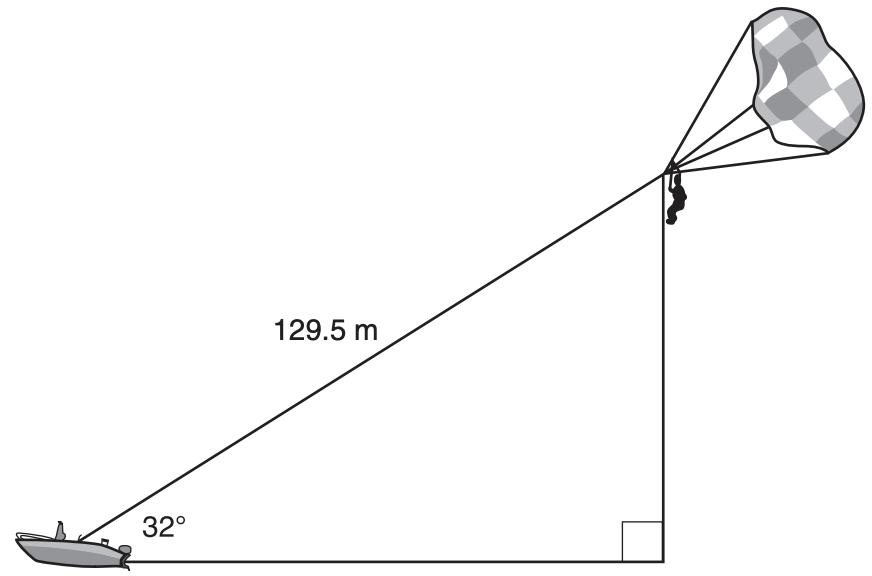
\includegraphics[width=9cm]{../graphics/parasail.png}
  \end{center}
If 129.5 meters of cable connected the boat to the parasail, approximately how many meters above the lake was the man? (to the \emph{nearest tenth of a meter})

\newpage
\item Regents problem \\
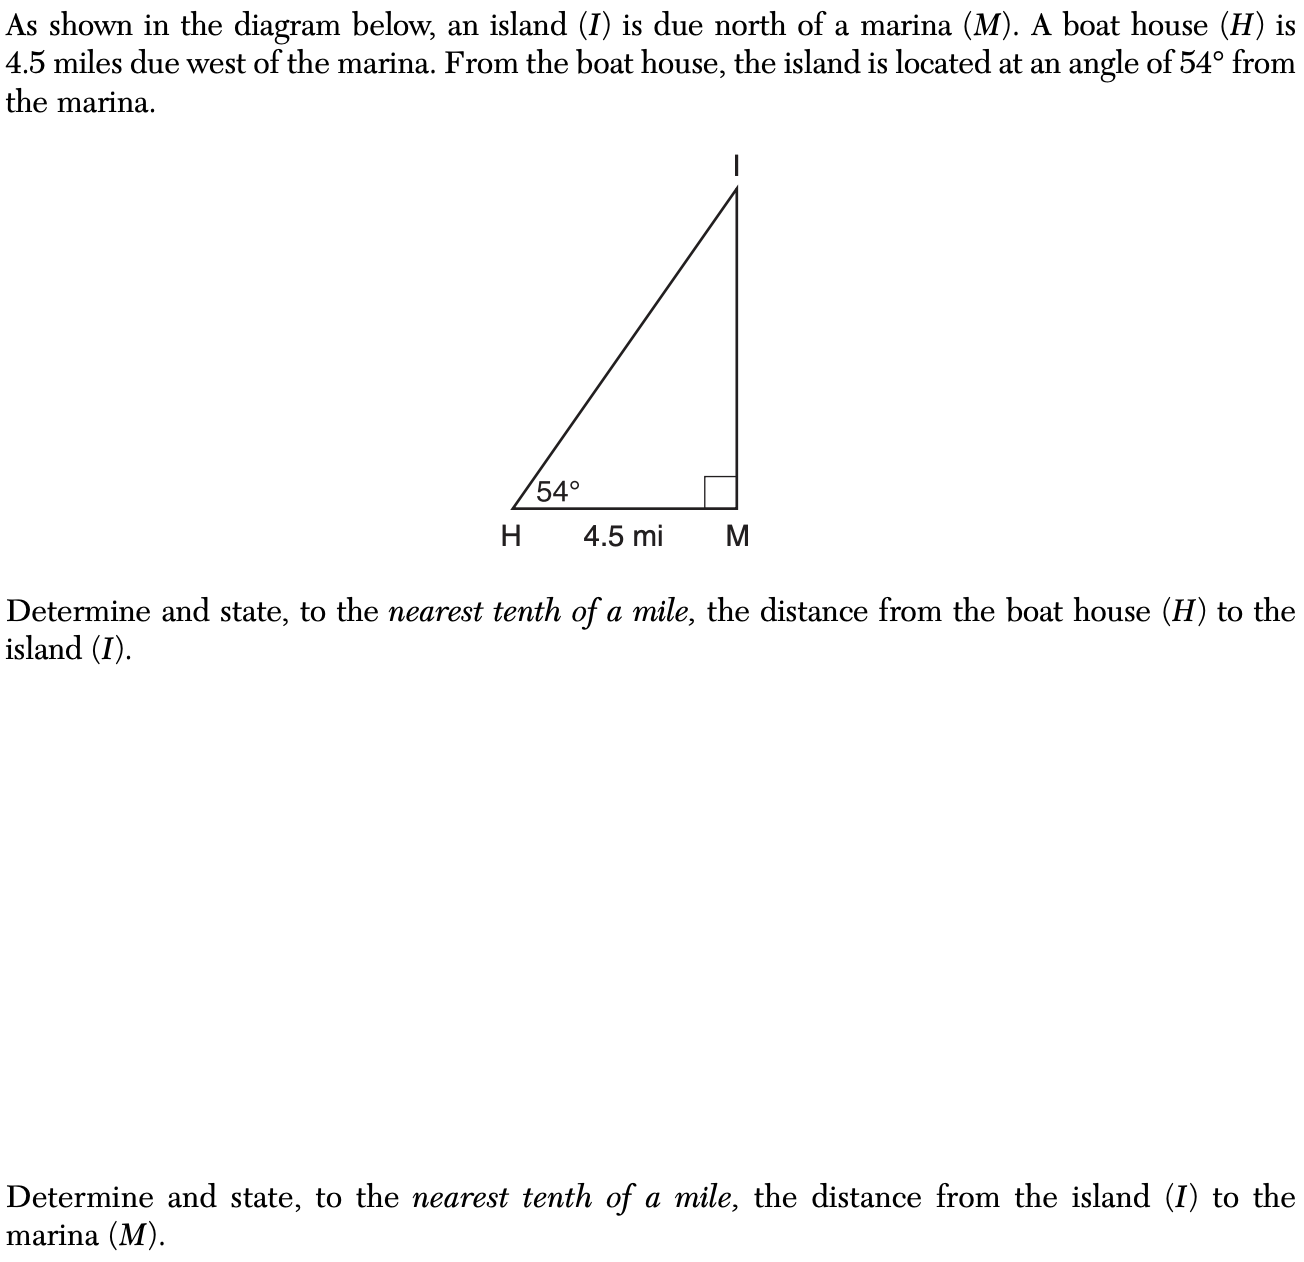
\includegraphics[width=16cm]{../graphics/marina.png}


\end{enumerate}
\end{document}
  